\begin{enumerate}[label=\thesection.\arabic*,ref=\thesection.\theenumi]
 \item  In each of the following cases, determine the direction cosines of the normal to
the plane and the distance from the origin.
\begin{enumerate}
	\item $z=2$ 
	\item $x + y + z = 1$
	\item $2x + 3y – z = 5$
	\item $5y + 8 = 0$
\end{enumerate}
    \solution
		\iffalse
\documentclass[12pt]{article}
\usepackage{graphicx}
\usepackage{amsmath}
\usepackage{mathtools}
\usepackage{gensymb}
\usepackage[utf8]{inputenc}
\usepackage{float}
\newcommand{\mydet}[1]{\ensuremath{\begin{vmatrix}#1\end{vmatrix}}}
\providecommand{\brak}[1]{\ensuremath{\left(#1\right)}}
\providecommand{\norm}[1]{\left\lVert#1\right\rVert}
\newcommand{\solution}{\noindent \textbf{Solution: }}
\newcommand{\myvec}[1]{\ensuremath{\begin{pmatrix}#1\end{pmatrix}}}
\let\vec\mathbf

\begin{document}
\begin{center}
\textbf\large{CLASS-12 \\ CHAPTER-11 \\ THREE DIMENSIONAL GEOMETRY}
\end{center}
\section*{Excercise 11.3}

\solution
\fi
\begin{enumerate}
\item From the given equation
	\begin{align}
		\vec{n}=\myvec{0\\0\\1},c=2
	\end{align}
	The distance from the origin is given by:
		\begin{align}
			d=\frac{|c|}{\norm{\vec{n}}}=\frac{2}{1}=2
		\end{align}

\item From the given equation
         \begin{align}
		\vec{n}=\myvec{1\\1\\1},c=1
			\end{align}
	 
	The distance from the origin is given by
		\begin{align}
			d=\frac{|c|}{\norm{\vec{n}}}=\frac{1}{\sqrt{3}}
		\end{align}

\item From the given equation
         \begin{align}
		\vec{n}=\myvec{2\\3\\-1},c=5
			\end{align}
	
	The distance from the origin is given by
		\begin{align}
			d=\frac{|c|}{\norm{\vec{n}}}=\frac{5}{\sqrt{14}}
		\end{align}
		
\item From the given equation
         \begin{align}
		\vec{n}=\myvec{0\\-5\\0},c=8
			\end{align}
	
	The distance from the origin is given by
		\begin{align}
			d=\frac{|c|}{\norm{\vec{n}}}=\frac{8}{5}
		\end{align}

\end{enumerate}
 


\item Find the vector equation of a plane which is at a distance of 7 units from the origin and normal to the vector $3\hat{i}+5\hat{j}-6\hat{k}$.
	\\
    \solution
		\iffalse
\documentclass[12pt]{article}
\usepackage{graphicx}
\usepackage[none]{hyphenat}
\usepackage{graphicx}
\usepackage{listings}
\usepackage[english]{babel}
\usepackage{graphicx}
\usepackage{caption} 
\usepackage{booktabs}
\usepackage{array}
\usepackage{amssymb} % for \because
\usepackage{amsmath}   % for having text in math mode
\usepackage{extarrows} % for Row operations arrows
\usepackage{listings}
\lstset{
  frame=single,
  breaklines=true
}
\usepackage{hyperref}
  
%Following 2 lines were added to remove the blank page at the beginning
\usepackage{atbegshi}% http://ctan.org/pkg/atbegshi
\AtBeginDocument{\AtBeginShipoutNext{\AtBeginShipoutDiscard}}


%New macro definitions
\newcommand{\mydet}[1]{\ensuremath{\begin{vmatrix}#1\end{vmatrix}}}
\providecommand{\brak}[1]{\ensuremath{\left(#1\right)}}
\providecommand{\norm}[1]{\left\lVert#1\right\rVert}
\newcommand{\solution}{\noindent \textbf{Solution: }}
\newcommand{\myvec}[1]{\ensuremath{\begin{pmatrix}#1\end{pmatrix}}}
\providecommand{\abs}[1]{\left\vert#1\right\vert}
\let\vec\mathbf

\begin{document}

\begin{center}
\title{\textbf{Equation  of Unit Vector}}
\date{\vspace{-5ex}} %Not to print date automatically
\maketitle
\end{center}
\setcounter{page}{1}
\section{12$^{th}$ Maths - Chapter 11}
\textbf{This is Problem-2 from Exercise 3.2}
\begin{enumerate}
\section{Solution}
\fi
From the given information, 
\begin{align} 
\vec{n}=\myvec{3\\5\\-6},\,
	d=\frac{\abs{c}}{\norm{\vec{n}}} = 7
\end{align}	  
yielding
\begin{align}
c =\pm7\sqrt{70}
\end{align}	  

	\item Find the equation of the plane with an intercept 3 on the Y-axis and parallel to ZOX-Plane.\\
    \solution
		\iffalse
\documentclass[A4,12pt,twocolumn]{IEEEtran}
%
\usepackage{setspace}
\usepackage{gensymb}
%\doublespacing
\singlespacing

%\usepackage{graphicx}
%\usepackage{amssymb}
%\usepackage{relsize}
\usepackage[cmex10]{amsmath}
%\usepackage{amsthm}
%\interdisplaylinepenalty=2500
%\savesymbol{iint}
%\usepackage{txfonts}
%\restoresymbol{TXF}{iint}
%\usepackage{wasysym}
\usepackage{amsthm}
%\usepackage{iithtlc}
\usepackage{mathrsfs}
\usepackage{txfonts}
\usepackage{stfloats}
\usepackage{bm}
\usepackage{cite}
\usepackage{cases}
\usepackage{subfig}
%\usepackage{xtab}
\usepackage{longtable}
\usepackage{multirow}
%\usepackage{algorithm}
%\usepackage{algpseudocode}
\usepackage{enumitem}
\usepackage{mathtools}
\usepackage{steinmetz}
\usepackage{tikz}
\usepackage{circuitikz}
\usepackage{verbatim}
\usepackage{tfrupee}
\usepackage[breaklinks=true]{hyperref}
%\usepackage{stmaryrd}
\usepackage{tkz-euclide} % loads  TikZ and tkz-base
%\usetkzobj{all}
\usetikzlibrary{calc,math}
\usepackage{listings}
    \usepackage{color}                                            %%
    \usepackage{array}                                            %%
    \usepackage{longtable}                                        %%
    \usepackage{calc}                                             %%
    \usepackage{multirow}                                         %%
    \usepackage{hhline}                                           %%
    \usepackage{ifthen}                                           %%
  %optionally (for landscape tables embedded in another document): %%
    \usepackage{lscape}     
\usepackage{multicol}
\usepackage{chngcntr}
%\usepackage{enumerate}

%\usepackage{wasysym}
%\newcounter{MYtempeqncnt}
\DeclareMathOperator*{\Res}{Res}
%\renewcommand{\baselinestretch}{2}
\renewcommand\thesection{\arabic{section}}
\renewcommand\thesubsection{\thesection.\arabic{subsection}}
\renewcommand\thesubsubsection{\thesubsection.\arabic{subsubsection}}

\renewcommand\thesectiondis{\arabic{section}}
\renewcommand\thesubsectiondis{\thesectiondis.\arabic{subsection}}
\renewcommand\thesubsubsectiondis{\thesubsectiondis.\arabic{subsubsection}}

% correct bad hyphenation here
\hyphenation{op-tical net-works semi-conduc-tor}
\def\inputGnumericTable{}                                 %%

\lstset{
%language=C,
frame=single, 
breaklines=true,
columns=fullflexible
}
%\lstset{
%language=tex,
%frame=single, 
%breaklines=true
%}

\begin{document}
%


\newtheorem{theorem}{Theorem}[section]
\newtheorem{problem}{Problem}
\newtheorem{proposition}{Proposition}[section]
\newtheorem{lemma}{Lemma}[section]
\newtheorem{corollary}[theorem]{Corollary}
\newtheorem{example}{Example}[section]
\newtheorem{definition}[problem]{Definition}
%\newtheorem{thm}{Theorem}[section] 
%\newtheorem{defn}[thm]{Definition}
%\newtheorem{algorithm}{Algorithm}[section]
%\newtheorem{cor}{Corollary}
\newcommand{\BEQA}{\begin{eqnarray}}
\newcommand{\EEQA}{\end{eqnarray}}
\newcommand{\define}{\stackrel{\triangle}{=}}

\bibliographystyle{IEEEtran}
%\bibliographystyle{ieeetr}


\providecommand{\mbf}{\mathbf}
\providecommand{\pr}[1]{\ensuremath{\Pr\left(#1\right)}}
\providecommand{\qfunc}[1]{\ensuremath{Q\left(#1\right)}}
\providecommand{\sbrak}[1]{\ensuremath{{}\left[#1\right]}}
\providecommand{\lsbrak}[1]{\ensuremath{{}\left[#1\right.}}
\providecommand{\rsbrak}[1]{\ensuremath{{}\left.#1\right]}}
\providecommand{\brak}[1]{\ensuremath{\left(#1\right)}}
\providecommand{\lbrak}[1]{\ensuremath{\left(#1\right.}}
\providecommand{\rbrak}[1]{\ensuremath{\left.#1\right)}}
\providecommand{\cbrak}[1]{\ensuremath{\left\{#1\right\}}}
\providecommand{\lcbrak}[1]{\ensuremath{\left\{#1\right.}}
\providecommand{\rcbrak}[1]{\ensuremath{\left.#1\right\}}}
\theoremstyle{remark}
\newtheorem{rem}{Remark}
\newcommand{\sgn}{\mathop{\mathrm{sgn}}}
\providecommand{\abs}[1]{\left\vert#1\right\vert}
\providecommand{\res}[1]{\Res\displaylimits_{#1}} 
\providecommand{\norm}[1]{\left\lVert#1\right\rVert}
%\providecommand{\norm}[1]{\lVert#1\rVert}
\providecommand{\mtx}[1]{\mathbf{#1}}
\providecommand{\mean}[1]{E\left[ #1 \right]}
\providecommand{\fourier}{\overset{\mathcal{F}}{ \rightleftharpoons}}
%\providecommand{\hilbert}{\overset{\mathcal{H}}{ \rightleftharpoons}}
\providecommand{\system}{\overset{\mathcal{H}}{ \longleftrightarrow}}
	%\newcommand{\solution}[2]{\textbf{Solution:}{#1}}
\newcommand{\solution}{\noindent \textbf{Solution: }}
\newcommand{\cosec}{\,\text{cosec}\,}
\providecommand{\dec}[2]{\ensuremath{\overset{#1}{\underset{#2}{\gtrless}}}}
\newcommand{\myvec}[1]{\ensuremath{\begin{pmatrix}#1\end{pmatrix}}}
\newcommand{\mydet}[1]{\ensuremath{\begin{vmatrix}#1\end{vmatrix}}}
%\numberwithin{equation}{section}
\numberwithin{equation}{subsection}
%\numberwithin{problem}{section}
%\numberwithin{definition}{section}
\makeatletter
\@addtoreset{figure}{problem}
\makeatother

\let\StandardTheFigure\thefigure
\let\vec\mathbf
%\renewcommand{\thefigure}{\theproblem.\arabic{figure}}
\renewcommand{\thefigure}{\theproblem}
%\setlist[enumerate,1]{before=\renewcommand\theequation{\theenumi.\arabic{equation}}
%\counterwithin{equation}{enumi}


%\renewcommand{\theequation}{\arabic{subsection}.\arabic{equation}}

\def\putbox#1#2#3{\makebox[0in][l]{\makebox[#1][l]{}\raisebox{\baselineskip}[0in][0in]{\raisebox{#2}[0in][0in]{#3}}}}
     \def\rightbox#1{\makebox[0in][r]{#1}}
     \def\centbox#1{\makebox[0in]{#1}}
     \def\topbox#1{\raisebox{-\baselineskip}[0in][0in]{#1}}
     \def\midbox#1{\raisebox{-0.5\baselineskip}[0in][0in]{#1}}

\vspace{3cm}


\title{GEOMETRY}
\author{Shristy Sharma (EE22BNITS11001)}





% make the title area
\maketitle

\newpage

%\tableofcontents

\bigskip

\renewcommand{\thefigure}{\theenumi}
\renewcommand{\thetable}{\theenumi}
%\renewcommand{\theequation}{\theenumi}


%Download all python codes 
%
%\begin{lstlisting}
%svn co https://github.com/JayatiD93/trunk/My_solution_design/codes
%\end{lstlisting}

%Download all and latex-tikz codes from 
%
%\begin{lstlisting}
%svn co https://github.com/gadepall/school/trunk/ncert/geometry/figs
%\end{lstlisting}
%


\section{PROBLEM 1}
SOLUTION:\\
\fi
The normal vector to the ZOX plane is
\begin{align} 
\vec{n} = \myvec{0\\1\\0}.
\end{align}
Since, Y-axis has the intercept 3, the desired plane passes through the point
\begin{align}
\vec{P}=\myvec{0\\3\\0}.
\end{align}
Thus, the equation of the plane is given by,
\begin{align}
	\vec{n}^\top \brak{\vec{x}-\vec{P}} &= 0\\
	\implies \myvec{0&1&0} \vec{x}&= 3
\end{align}
See Fig. 
     \ref{fig:chapters/12/11/3/8/1}.
\begin{figure}[h!]
  \centering
   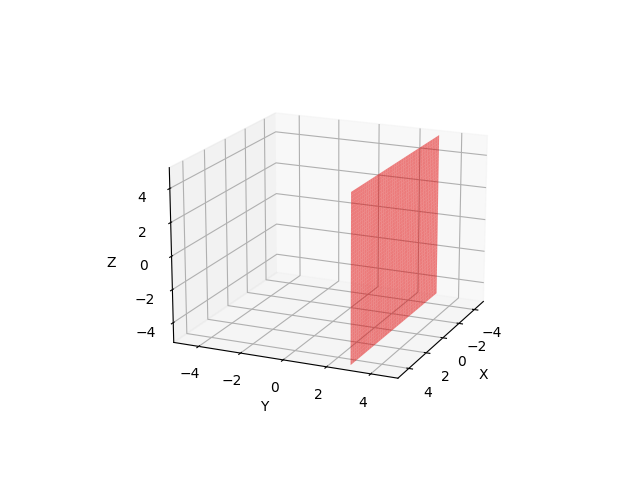
\includegraphics[width=\columnwidth]{chapters/12/11/3/8/figs/plane1.png}
    \caption{}
     \label{fig:chapters/12/11/3/8/1}
     \end{figure}  

\item In the following cases, determine whether the given planes are parallel or perpendicular, and in case they are neither, find the angles between them.
\begin{enumerate}
\item $7x + 5y + 6z + 30 = 0$ and $3x – y – 10z + 4 = 0$
\item $2x + y + 3z – 2 = 0$ and $x – 2y + 5 = 0$
\item $2x – 2y + 4z + 5 = 0$ and $3x – 3y + 6z – 1 = 0$
\item $2x – y + 3z – 1 = 0$ and $2x – y + 3z + 3 = 0$
\item $4x + 8y + z – 8 = 0$ and $y + z – 4 = 0$
\end{enumerate}
    \solution
		\iffalse
\documentclass[journal,12pt,twocolumn]{IEEEtran}
\usepackage{romannum}
\usepackage{float}
\usepackage{setspace}
\usepackage{gensymb}
\singlespacing
\usepackage[cmex10]{amsmath}
\usepackage{amsthm}
\usepackage{mathrsfs}
\usepackage{txfonts}
\usepackage{stfloats}
\usepackage{bm}
\usepackage{cite}
\usepackage{cases}
\usepackage{subfig}
\usepackage{longtable}
\usepackage{multirow}
\usepackage{enumitem}
\usepackage{mathtools}
\usepackage{steinmetz}
\usepackage{tikz}
\usepackage{circuitikz}
\usepackage{verbatim}
\usepackage{tfrupee}
\usepackage[breaklinks=true]{hyperref}
\usepackage{tkz-euclide}
\usetikzlibrary{calc,math}
\usepackage{listings}
    \usepackage{color}                                            %%
    \usepackage{array}                                            %%
    \usepackage{longtable}                                        %%
    \usepackage{calc}                                             %%
    \usepackage{multirow}                                         %%
    \usepackage{hhline}                                           %%
    \usepackage{ifthen}                                           %%
  %optionally (for landscape tables embedded in another document): %%
    \usepackage{lscape}     
\usepackage{multicol}
\usepackage{chngcntr}
\DeclareMathOperator*{\Res}{Res}
\renewcommand\thesection{\arabic{section}}
\renewcommand\thesubsection{\thesection.\arabic{subsection}}
\renewcommand\thesubsubsection{\thesubsection.\arabic{subsubsection}}

\renewcommand\thesectiondis{\arabic{section}}
\renewcommand\thesubsectiondis{\thesectiondis.\arabic{subsection}}
\renewcommand\thesubsubsectiondis{\thesubsectiondis.\arabic{subsubsection}}

% correct bad hyphenation here
\hyphenation{op-tical net-works semi-conduc-tor}
\def\inputGnumericTable{}                                 %%

\lstset{
frame=single, 
breaklines=true,
columns=fullflexible
}

\begin{document}


\newtheorem{theorem}{Theorem}[section]
\newtheorem{problem}{Problem}
\newtheorem{proposition}{Proposition}[section]
\newtheorem{lemma}{Lemma}[section]
\newtheorem{corollary}[theorem]{Corollary}
\newtheorem{example}{Example}[section]
\newtheorem{definition}[problem]{Definition}
\newcommand{\BEQA}{\begin{eqnarray}}
\newcommand{\EEQA}{\end{eqnarray}}
\newcommand{\define}{\stackrel{\triangle}{=}}

\bibliographystyle{IEEEtran}
\providecommand{\mbf}{\mathbf}
\providecommand{\pr}[1]{\ensuremath{\Pr\left(#1\right)}}
\providecommand{\qfunc}[1]{\ensuremath{Q\left(#1\right)}}
\providecommand{\sbrak}[1]{\ensuremath{{}\left[#1\right]}}
\providecommand{\lsbrak}[1]{\ensuremath{{}\left[#1\right.}}
\providecommand{\rsbrak}[1]{\ensuremath{{}\left.#1\right]}}
\providecommand{\brak}[1]{\ensuremath{\left(#1\right)}}
\providecommand{\lbrak}[1]{\ensuremath{\left(#1\right.}}
\providecommand{\rbrak}[1]{\ensuremath{\left.#1\right)}}
\providecommand{\cbrak}[1]{\ensuremath{\left\{#1\right\}}}
\providecommand{\lcbrak}[1]{\ensuremath{\left\{#1\right.}}
\providecommand{\rcbrak}[1]{\ensuremath{\left.#1\right\}}}
\theoremstyle{remark}
\newtheorem{rem}{Remark}
\newcommand{\sgn}{\mathop{\mathrm{sgn}}}
\providecommand{\abs}[1]{\left\vert#1\right\vert}
\providecommand{\res}[1]{\Res\displaylimits_{#1}} 
\providecommand{\norm}[1]{\left\lVert#1\right\rVert}
\providecommand{\mtx}[1]{\mathbf{#1}}
\providecommand{\mean}[1]{E\left[ #1 \right]}
\providecommand{\fourier}{\overset{\mathcal{F}}{ \rightleftharpoons}}
\providecommand{\system}{\overset{\mathcal{H}}{ \longleftrightarrow}}
\newcommand{\solution}{\noindent \textbf{Solution: }}
\newcommand{\cosec}{\,\text{cosec}\,}
\providecommand{\dec}[2]{\ensuremath{\overset{#1}{\underset{#2}{\gtrless}}}}
\newcommand{\myvec}[1]{\ensuremath{\begin{pmatrix}#1\end{pmatrix}}}
\newcommand{\mydet}[1]{\ensuremath{\begin{vmatrix}#1\end{vmatrix}}}
\numberwithin{equation}{subsection}
\makeatletter
\@addtoreset{figure}{problem}
\makeatother

\let\StandardTheFigure\thefigure
\let\vec\mathbf
\renewcommand{\thefigure}{\theproblem}



\def\putbox#1#2#3{\makebox[0in][l]{\makebox[#1][l]{}\raisebox{\baselineskip}[0in][0in]{\raisebox{#2}[0in][0in]{#3}}}}
     \def\rightbox#1{\makebox[0in][r]{#1}}
     \def\centbox#1{\makebox[0in]{#1}}
     \def\topbox#1{\raisebox{-\baselineskip}[0in][0in]{#1}}
     \def\midbox#1{\raisebox{-0.5\baselineskip}[0in][0in]{#1}}

\vspace{3cm}


\title{Assignment 1}
\author{Jaswanth Chowdary Madala}





% make the title area
\maketitle

\newpage

%\tableofcontents

\bigskip

\renewcommand{\thefigure}{\theenumi}
\renewcommand{\thetable}{\theenumi}

\begin{enumerate}

\textbf{Solution:} 
\fi
		The angle between the planes is the angle between the normals of the given planes.
\begin{align}
\vec{n_1}^{\top}\vec{x} = c_1, \, \vec{n_2}^{\top}\vec{x} &= c_2
\end{align}
The angle $\theta$ between the planes is given by,
\begin{align}
\cos{\theta} &= \frac{\vec{n_1}^{\top}\vec{n_2}}{\norm{\vec{n_1}}\norm{\vec{n_2}}}
\end{align}

\begin{enumerate}
\item
\begin{align}
\vec{n_1} = \myvec{7\\5\\6}, \, \vec{n_2} &= \myvec{3\\-1\\-10}\\
\implies \vec{n_1}^{\top}\vec{n_2} = \myvec{7&5&6}\myvec{3\\-1\\-10}
	&= -44\\
\norm{\vec{n_1}} = \sqrt{7^2+5^2+6^2}
&= \sqrt{110}\\
\norm{\vec{n_2}} = \sqrt{3^2+\brak{-1}^2+\brak{-10}^2} 
&= \sqrt{110}\\
\cos{\theta} = -\frac{44}{\sqrt{110}\sqrt{110}}
&= -\frac{2}{5}
\end{align}
The planes are inclined at an angle of $\arccos\brak{{-\frac{2}{5}}}$ degrees.

\item
\begin{align}
\vec{n_1} = \myvec{2\\1\\3},\, \vec{n_2} &= \myvec{1\\-2\\0}\\
\vec{n_1}^{\top}\vec{n_2} = \myvec{2&1&3}\myvec{1\\-2\\0}\\
= 0
\end{align}  
The planes are perpendicular.
\item
\begin{align}
\vec{n_1} = \myvec{2\\-2\\4},\, \vec{n_2} &= \myvec{3\\-3\\6}\\
\vec{n_1}^{\top}\vec{n_2} = \myvec{2&-2&4}\myvec{3\\-3\\6}
&= 36\\
\norm{\vec{n_1}} = \sqrt{2^2+\brak{-2}^2+4^2}
&= \sqrt{24}\\
\norm{\vec{n_2}} = \sqrt{3^2+\brak{-3}^2+6^2} 
&= \sqrt{54}\\
\cos{\theta}= \frac{36}{\sqrt{24}\sqrt{54}}\\
&= 1
\end{align}
The planes are parallel.
\item
\begin{align}
\vec{n_1} = \myvec{2\\-1\\3}, \, \vec{n_2} &= \myvec{2\\-1\\3}\\
\vec{n_1}^{\top}\vec{n_2} = \myvec{2&-1&3}\myvec{2\\-1\\3}
&= 14\\
\norm{\vec{n_1}} &= \sqrt{2^2+\brak{-1}^2+3^2}
&= \sqrt{14}\\
\norm{\vec{n_2}} = \sqrt{2^2+\brak{-1}^2+3^2}
&= \sqrt{14}\\
\cos{\theta} = \frac{14}{\sqrt{14}\sqrt{14}}
&= 1
\end{align}
The planes are parallel.
\item
\begin{align}
\vec{n_1} = \myvec{4\\8\\1}, \, \vec{n_2} &= \myvec{0\\1\\1}\\
\vec{n_1}^{\top}\vec{n_2} = \myvec{4&8&1}\myvec{0\\1\\1}
&= 9\\
\norm{\vec{n_1}} = \sqrt{4^2+8^2+1^2}
&= 9\\
\norm{\vec{n_2}} = \sqrt{0^2+1^2+1^2} 
&= \sqrt{2}\\
\cos{\theta} = \frac{9}{9\sqrt{2}}
&= \frac{1}{\sqrt{2}}
\end{align}
The planes are inclined at an angle of 45 degrees.
\end{enumerate}

\end{enumerate}

